\section{Správa paměti, statické přidělování paměti, dynamické přidělování paměti, garbage collector, reprezentace informace v paměti.}
Každá paměť, která je přiřazena procesu se dělí na 4 základní bloky:
\begin{multicols}{2}
\begin{itemize}
    \item Segment instrukcí(Code)/Kódová oblast
    \item Datový segment(Data)/Datová oblast
    \item Halda/hromada(Heap)
    \item Zásobník(Stack)
    \vfill
\end{itemize}
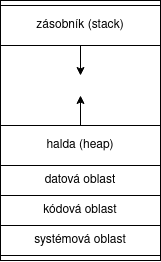
\includegraphics[scale=0.3]{BPC-TIN/images/pamet.png}
\end{multicols}
\textbf{Code}\,--\,je to množina strojových instrukcí, které naprosto jednoznačně provádí program. Dle těchto instrukcí PC postupuje ve výpočtu.

\textbf{Data}\,--\,v této části můžou být uložena data, která jsou známa při překladu programu (Hodnoty polí, konstant, proměnných, nějaké textové řetězce).

 Bloky Code a Data jsou známy v době překladu a jejich velikost se v průběhu nemění.

\textbf{Heap}\,--\,slouží k alokaci dynamické paměti. Je založena na stromové datové struktuře. Obsahuje objekty a instance proměnných(atributy třídy).

\textbf{Stack}\,--\,je důležitý pro volaní správné funkcí. Funguje na principu LIFO. Funguje tak že se ukládají funkce do stacku, se kterými se posunuje taktéž ukazatel na pozici v registeru. Po dokončení té funkce je odstraněna ze zásobníku a ukazatel změněn na předchozí funkci. Obsahuje metody/funkce, lokální proměnné a reference na proměnné. Video pro lepší vysvětlení \url{https://www.youtube.com/watch?v=uwV0hotRrLw}.

 Bloky Heap a Stack jsou dynamické a jejich velikost roste/zmenšuje u každého z jiným směrem v průběhu programu.

\begin{Large}\vspace{0,5cm} \textbf{Statické přidělování paměti}
\end{Large}

 Staticky se ukládají datové struktury, které jsou definovány při překladu programu. K jednotlivým paměťovým úsekům lze přistupovat pomocí názvu proměnné. V průběhu se adresa nemůže měnit.

\begin{Large}\vspace{0,5cm} \textbf{Dynamické přidělování paměti}
\end{Large}

 Dynamicky se paměť přiděluje na základě požadavku při průběhu programu. K dynamicky přidělenému paměťovému úseku se dá přistoupit pouze nepřímo pomocí ukazatele. Ukazatel je součástí statické nebo dynamické struktury. Dynamicky přidělovaná paměť se čerpá z vyhrazeného prostoru paměti počítače.

\begin{Large}\vspace{0,5cm} \textbf{Dynamické přidělování paměti bez regenerace}
\end{Large}

 Regenerace paměti je její pročištění od nepoužívaných částí paměti.

 Dynamické přidělovaní paměti bez regenerace přiděluje požadované úseky postupně tak jak jsou za sebou umístěny až do vyčerpaní vyhrazené paměti. Využívá pracovního ukazatele, který ukazuje na první adresu volné paměti. Nejčastěji pomocí operace "new" zapíše do paměti a změní ukazatel na novou hodnotu, která ukazuje na novou adresu volné části a v indikátoru paměti hodnotu obsazení označí true. Operace "free/delete" okamžitě neuvolní paměť, ale přepíše indikátor paměti na false. Kdy pak regenerace probíhá po větších částech. 

\begin{Large}\vspace{0,5cm} \textbf{Dynamické přidělování paměti s regenerací}
\end{Large}

 Na rozdíl od dynamického přidělovaní bez regenerací se zde regeneruje pro každé operaci "free/delete". S tím přichází problém s fragmentací paměti. Po uvolnění paměti by tyto části mohli vytvářet sekvence malých, oddělených a přitom sousedních prvků. Často je defragmentace těchto volných bloků spojena s operací "free/delete". Snaží se slučovat volné úseky se sousedními volnými úseky.

\begin{Large}\vspace{0,5cm} \textbf{Garbage collector}
\end{Large}

 Je nejpokročilejším způsobem dynamického přidělovaní paměti. Oproti předchozím způsobům je méně efektivní. 
Skládá se ze tří fází:
\begin{itemize}
    \item \textbf{Allocation}\,--\,přiděluje po sobě jdoucí úseky stejně jako metoda bez regenerace až do vyčerpání celého vyhrazeného prostoru.
    \item\textbf{Marking}\,--\,nastává pouze pokud je vyčerpán celý prostor. Prochází prostorem a vyhledává a označuje úseky, které nejsou aktivní a jejich návrat do společné paměti způsobí regeneraci.
    \item\textbf{Garbage collecting}\,--\,provádí se defragmentace přesunem všech uvolněných úseků do jednoho souvislého úseku. Tím se vytvoří nový souvislý úsek pro alokaci.
\end{itemize}

 Tyto tři fáze se opakují dokola, dokud nedojde k situaci, že nový úsek není dostačující pro fázi alokace. Z tohoto důvodu dojde k ukončení programu.

\vspace{1cm}
\textbf{Reprezentace informace v paměti}\,--\,pokud je datový typ primitivní je uložen na přímo v paměti a u objektů je reprezentován pouze ukazatelem na místo v paměti.







\newpage
\section{Jazyk UML a objektově orientovaný návrh - dědičnost, generalizace, asociace 1:n, n:1, n:n, agregace a kompozice.}

 \textbf{Jazyk UML} je grafický jazyk pro popis programových systémů. Slouží pro vizualizaci, specifikaci, návrh a dokumentaci systémů. K zobrazení se využívají diagramy, kde nejčastěji používané jsou:
\begin{enumerate}
    \item Strukturální
    \begin{enumerate}
        \item Diagram tříd
        \item Diagram případů užití
        \item Diagram komponent
        \item Diagram nasazení
    \end{enumerate}
    \item Behaviorální
    \begin{enumerate}
        \item Diagram aktivit
        \item Diagram sekvencí
        \item Diagram stavů.
    \end{enumerate}
\end{enumerate}
Nejpoužívanější jsou diagramy tříd a případů užití. Diagram tříd popisuje strukturu systému, znázorňuje datové struktury a operace u objektů a souvislosti mezi nimi. Skládá se z tříd, rozhraní, abstraktních tříd. Tyto tři prvky se dále skládají z názvu třídy/rozhraní, atributů (rozhraní neobsahuje atributy), a operace (metody/funkce) Diagram případů užití se nejčastěji používá při komunikaci se zákazníkem a méně technicky znalou stranou. Skládá se z herců (actor) a případů užití a systém. Tyto strany jsou propojeny jak mezi sebou tak i sami se sebou pomocí těchto propojení\,--\,asociace, generalizace, rozšíření vztahu, vztah zahrnuje

\textbf{Objektově orientovaný návrh} je jeden ze způsobů jak reprezentovat informaci. Vychází z principů reálného světa, neboli je jednoduše srozumitelný pro člověka. Není spojen s žádným programovacím jazykem ale jazyk, který bude použit pro implementaci musí splňovat objektově orientované principy. Výhodou OO návrhu může být, že při návrhu lze určit co jaká část programu komunikuje z jakou a co každá dělá, takže se sníží počet chyb v kódu a tím i náklady. OO návrh se nezabývá konkrétní implementací ale pouze vazbami mezi objekty.

Kdy není vhodný OO přístup? Není vhodné ho použít jestliže na cílové platformě neexistuje překladač OO jazyka. Nebo potřebuji to v jazyce, který nepodporuje OOP. Přepis stávající kódu by byl neekonomický, hlavně u projektů s krátkou životností.

\begin{Large}\vspace{0,5cm} \textbf{Vztahy mezi třídami}
\end{Large}

\textbf{Závislost}\,--\, je dynamický a zároveň nejslabší vztah. Ukazuje jak co na sobě závisí.\\
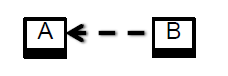
\includegraphics[scale=1]{BPC-TIN/images/zavislost.PNG}

\textbf{Asociace}\,--\, je pevný vztah. Určuje vztah mezi dvěma prvky, které mohou existovat nezávisle na sobě. Asociace může mít směr od jednoho prvku k druhému nebo obousměrně. Objekt ve směru šipky může nalézt odkaz na následujíc objekty. \\
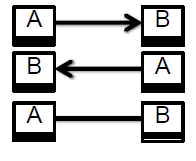
\includegraphics[scale=1]{BPC-TIN/images/asociace.PNG}

\textbf{Násobnost asociací}\,--\, určuje kolik vazeb může mít danný objekt. Například 1:n může být 1 objekt a ten mít reference na n objektů ke kterým má asociaci (faktura:n * položka).

\textbf{Agregace}\,--\, je typ asociace. reprezentuje vztah typu celek--část. Zde je u celku umístěn kosočtverec. Celek je entita, která drží kolekci prvků. Část může existovat bez celku nebo být součástí jiných kolekcí. \\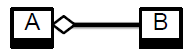
\includegraphics[scale=1]{BPC-TIN/images/agregace.PNG}

\textbf{Kompozice}\,--\, je typ asociace. Je to nejsilnější vztah a je podobná agregaci. S rozdílem v tom že část nemá bez celku smysl. pokud zanikne celek zaniknou i části. U celku je násobnost vždy 1.\\ 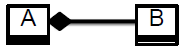
\includegraphics[scale=1]{BPC-TIN/images/kompozice.PNG}

\textbf{Dědičnost/generalizace}\,--\,se využívá jestliže mají některé třídy společné vlastnosti. Tím například nemusíme vytvářet duplicitní kód. Směr šipky udává od koho třída dědí (obrázek b dědí z a). Díky tomuto lze jednodušeji rozšířit třídu o atributy a operace. Neplést si z asociací nijak nesouvisí.\\
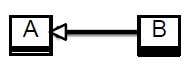
\includegraphics[scale=1]{BPC-TIN/images/dedicnost.PNG}






\newpage
\section{Třídy složitosti paměťové a časové. Notace Theta. Notace Omega. Notace velké-O. Asymptotický popis složitosti algoritmu. Posouzení složitosti známých algoritmů řazení. Posouzení složitosti algoritmu vyhledávání. Srovnání lineárních a nelineárních struktur. Vztah časové a paměťové složitosti.}

Složitost je vztah algoritmu k prostředkům (čas a velikost paměti). Paměťová složitost je závislost paměťových nároků na vstupních datech. Zatímco časová je dána hrubým odhadem počtu kroků, který daný algoritmus musí provést na základě délky vstupních dat.

\begin{Large}\vspace{0,5cm} \textbf{Asymptotická složitost}
\end{Large}

Jelikož ne vždy lze určit přesnou složitost algoritmu tak byla vyvinuta asymptotická složitost. Tato složitost aproximuje chovaní funkce ze tří pohledu:
\begin{itemize}
    \item Nejlepší případ $\Omega$ (Omega)\,--\,značí spodní hranici trvání algoritmu.
    \item Průměrný případ $\Theta$ (Theta)\,--\,odhaduje nejpravděpodobnější dobu trvání algoritmu.
    \item Nejhorší případ notace O (Omicron, big-O)\,--\,značí horní hranici trvání algoritmu. Je nejčastěji používaná.
\end{itemize}

\begin{table}[h]
    \begin{tabularx}{\textwidth}{|c|c|X|}\hline
        Konstantní & O(1) & Nezávisí na velikosti vstupních dat\\\hline
        Logaritmická & O($\log{n}$) & Počet operací odpovídá logaritmu např. vstup 1\,000\,000\,000 $==$ 30 operací\\\hline
        Lineární & O($n$)& počet operací je závislý na velikosti vstupních dat\\\hline
        Kvazilineární& O($n\log{n}$)& Zástupce quicksort\\\hline
        Kvadratická& O($n^2$)& Např 500 vstupů $==$ 250\,000 operací\\\hline
        Kubická & O($n^3$)& Např. 200 vstupů $==$ 8\,000\,000 operací\\\hline
        Exponenciální&O($2^n$)& Exponenciální růst počtu operací\\\hline
        Faktoriální&O($n!$)& Faktoriální růst počtu operací\\\hline
    \end{tabularx}
\end{table}

\textbf{Polynomiální algoritmy}\,--\,Jsou takové algoritmy jejichž notace v big-O je ohraničena polynomiální funkcí shora. Spadají zde například $\log{n}$, $k*n$, $3n^3 + 4n$, $2*n\log{n}$ a podobné. Nepatří sem exponenciální, faktoriální a jim podobné. Abychom algoritmus označili jako efektivní jeho vykonání by mělo být možné v polynomiálním čase jinak ho lze označit jako neefektivní. Při vysokých hodnotách v kryptografii by ne-polynomiální algoritmy byli nepoužitelné.

\begin{Large}\vspace{0,5cm} \textbf{Algoritmy řazení.}
\end{Large}

Třídění pomocí algoritmů Bubble Sort, Insert Sort a Select Sort má složitost O($n^2$). Algoritmus Quick Sort má složitost $\theta$($n\log{n}$), kdy v nejhorším případě může nabývat až O($n^2$). Algoritmus Merge Sort má složitost O($n\log{n}$).

\vspace{1cm}
\begin{Large}\vspace{0,5cm} \textbf{Lineární a nelineární struktury.}
\end{Large}

\textbf{Lineární}\,--\,zde spadají pole, seznamy, zásobník, fronta.
\begin{table}[h]
    \centering
    \begin{tabular}{|c|c|c|c|c|}\hline
         Struktura & Přidat & Vyhledat & Smazat & Výběr dle indexu\\\hline
         Pole & O($n$) & O($n$) & O($n$) & O($1$) \\\hline
         Seznam & O($1$) & O($n$) & O($n$) & O($n$)\\\hline
         Pole proměnlivé délky & O($1$) & O($n$) & O($n$) & O($1$) \\\hline
         Zásobník & O($1$) & -- & O($1$) & -- \\\hline
         Fronta & O($1$) & -- & O($1$) & -- \\\hline
    \end{tabular}
\end{table}

\textbf{Nelineární}\,--\,zde můžou spadat stromy, které pokud jsou nějak vyvažovány, tak mají náročnost O($\log{n}$). Pokud se nevyvažují tak náročnost je O($n$).

\begin{Large}\vspace{0,5cm} \textbf{Vztah časové a paměťové složitosti.}
\end{Large}

Většina algoritmů je kompromisem mezi těmito dvěma druhy složitosti. Pokud bychom měli algoritmus s vysokými nároky na časovou složitost (aby byl co nejrychlejší) tak jeho paměťová složitost bude vzrůstat. Většinu algoritmů je nějakým způsobem optimalizovaná nebo ji lze optimalizovat.

\begin{Large}\vspace{0,5cm} \textbf{Třídy složitosti}
\end{Large}

Vyjadřuje jak náročný je výpočet je nezbytný k vyřešení problému.\\
Rozdělení:
\begin{itemize}
    \item Třída P\,--\,schůdné algoritmy. Jsou proveditelné v polynomiálním čase na deterministickém turingově stroji.
    \item Třída NP\,--\,neschůdné algoritmy. Je možné je provést v polynomiálním čase na \textbf{nedeterministickém} TS (nebyl doposud sestaven). Spadají pod ně i všechny algoritmy z třídy P
    \item Třída NP-těžké\,--\,přinejmenším tak těžké, jako nejtěžší z NP. Nemusí být vykonatelné pomocí TS.
\end{itemize}









\newpage
\section{Abstraktní datový typ (ADT). ADT lineární seznam. ADT cyklický seznam. Operace vkládání, mazání a~vyhledávání prvku v ADT lineární seznam. ADT zásobník, ADT fronta.}

Abstraktní datový typ je množina druhů dat (hodnot) a příslušných operací, které jsou přesně specifikovány a to nezávisle na konkrétní implementaci. Zjednodušeně ADT je reprezentováno rozhraním, kde uživatele tohoto rozhraní zajímá pouze, jak se používá a ne jak je implementováno. Poté co je konkrétní ADT implementován v programovacím jazyce stává se z něj datová struktura.

ADT dělíme podle počtu datových položek na statický a dynamický datový typ. Statický datový typ má neměnnou velikost a dynamický mění velikost dle provedené operace. Dále se dělí jestli mají jednoznačného bezprostředního následníka na lineární a nelineární. Lineární mají následníka a u nelineárních neexistuje přímý jednoznačný následník.

\textbf{Dělení ADT:}
\begin{itemize}
    \item Lineární
    \begin{itemize}
        \item Pole\,--\,statický
        \item Seznam\,--\,dynamický
        \item Zásobník\,--\,dynamický
        \item Fronta\,--\,dynamický
    \end{itemize}
    \item Nelineární
    \begin{itemize}
        \item Strom\,--\,dynamický
        \item Množina (Set)\,--\,dynamický
    \end{itemize}
\end{itemize}

\begin{Large}\vspace{0,5cm} \textbf{Lineární seznam}
\end{Large}

ADT lineární seznam je seznam, kde každý uzel má unikátního následníka.
Výhodou lineárního seznamu je že má efektivní vkládání a mazání ale neefektivní přístup k prvkům. Na rozdíl od pole, kde je rychlá indexace prvků. Každý prvek obsahuje data a ukazatel na další prvek v seznamu.
\begin{center}
    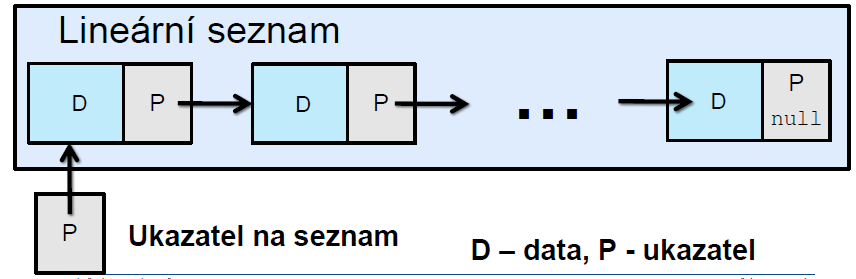
\includegraphics[scale=0.5]{BPC-TIN/images/linsez.PNG}
\end{center}

Možné operace s ADT seznamem:
\begin{itemize}
    \item Nalezení délky N seznamu
    \item Výpis všech prvků seznamu
    \item Vytvoření prázdného seznamu
    \item Získaní k-tého prvku ze seznamu
    \item Vložení novéhé prvku za k-tý prvek seznamu
    \item Smazaní prvku ze seznamu
    \item Nalezení následujícího prvku za aktuálním v seznamu
    \item Nalezení předchozího prvku před aktuálním v seznamu
\end{itemize}

\textbf{Cyklický lineární seznam}\,--\,stejný jako lineární ale poslední prvek nemá ukazatel null ale odkaz na první prvek seznamu.

\begin{center}
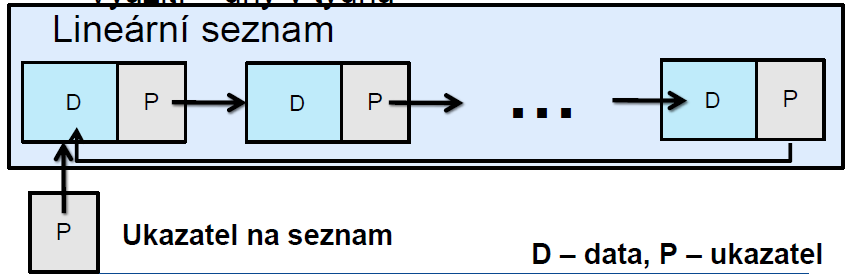
\includegraphics[scale=0.5]{BPC-TIN/images/cycsez.PNG}
\end{center}

\textbf{Obousměrně vázaný lineární seznam}\,--\,nemá pouze ukazatel na další prvek ale i na předchozí. Umožňuje procházení v obou směrech.

\begin{center}
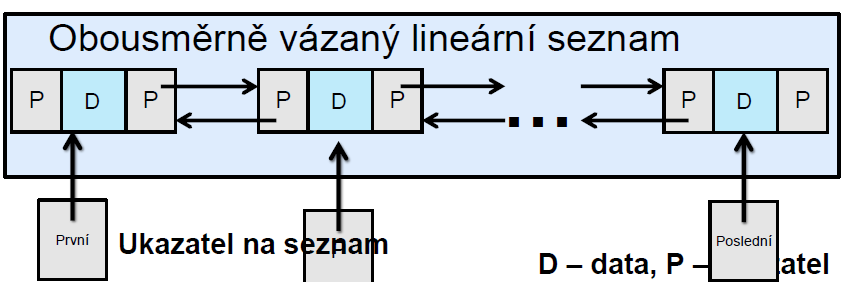
\includegraphics[scale=0.5]{BPC-TIN/images/obousez.PNG}
\end{center}

\textbf{Vkládaní do lineárního seznamu}\,--\,vložit prvek na určitou pozici funguje tak, že se najde pozice k kde se zde vloží prvek který bude odkazovat na prvek, který byl předtím na pozici k a v prvku k-1 se přepíše ukazatel na nový prvek. Operace fungují stejně jen jsou vázány na obě strany.

\begin{center}
    
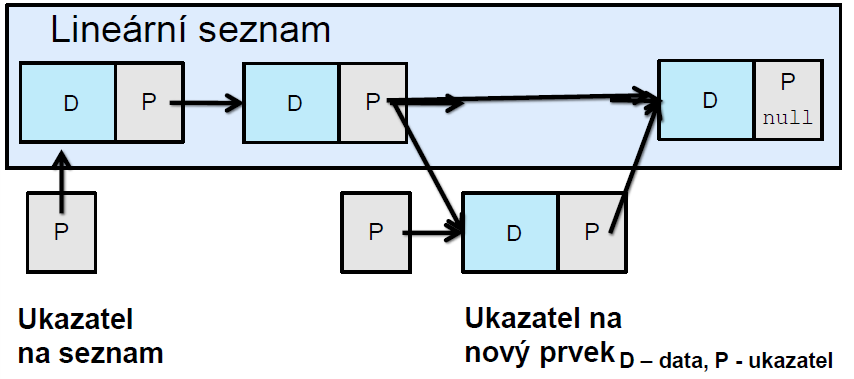
\includegraphics[scale=0.5]{BPC-TIN/images/sezins.PNG}
\end{center}

Pokud vkládáme na začátek tak se přepisuje ukazatel pole na první prvek a ve vkládaném prvku se přidá ukazatel na předchozí první prvek.

\begin{center}
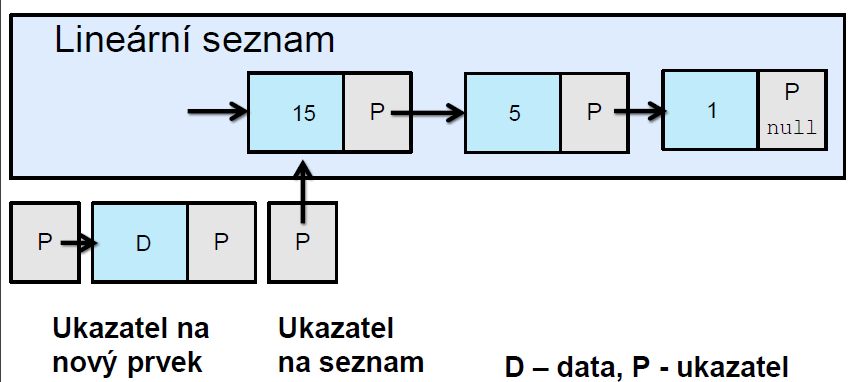
\includegraphics[scale=0.5]{BPC-TIN/images/sezinsfirst.PNG}

\vspace{1cm}
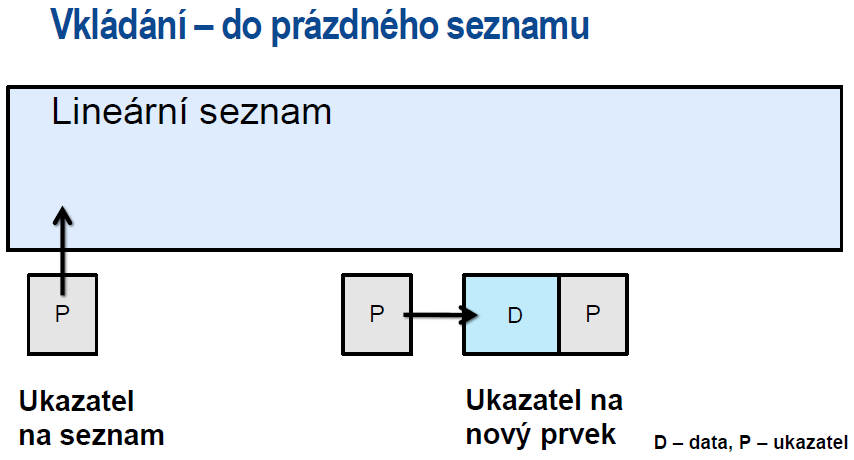
\includegraphics[scale=0.5]{BPC-TIN/images/sezinsempty.PNG}
\end{center}

\textbf{Mazaní v lineárním seznamu}\,--\,mazaní prvku na pozici k funguje tak že prvek k-1 přepíše ukazatel na prvek k+1. U prvního prvku se přepíše pouze ukazatel na další prvek.
\begin{center}
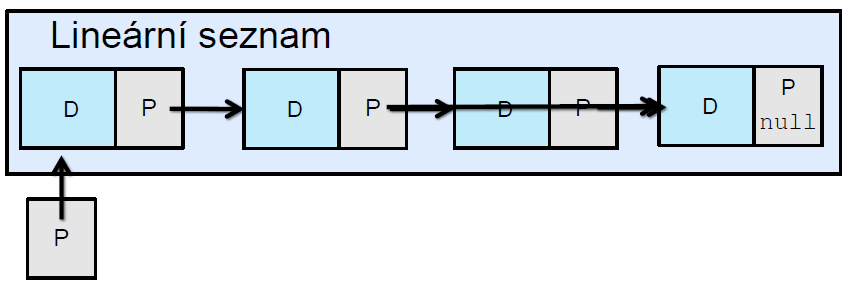
\includegraphics[scale=0.5]{BPC-TIN/images/sezdel.PNG}
\end{center}

\textbf{Vyhledávaní v lineárním seznamu}\,--\,dá se vyhledávat podle prvku nebo podle dat. Pomalu iteruje seznamem dokud nenarazí na ten prvek nebo konec seznamu. U obousměrného se dá hledat od začátku a od konce.

\begin{Large}\vspace{0,5cm} \textbf{Zásobník}
\end{Large}

Je dynamická datová struktura umožnující vkládaní a odebírání hodnot tak, že naposledy vložená hodnota se odebere jako první (LIFO). Základní operace jsou Vložený na vrchol, odebraní z vrcholu a test na prázdnost zásobníku. 

\begin{Large}\vspace{0,5cm} \textbf{Fronta}
\end{Large}

Je dynamická datová struktura, kde se odebírají prvky v tom pořadí v jakém byli vloženy (FIFO). Základní operace jsou stejné jako u zásobníku. Existuje tzv. prioritní fronta, která funguje na principu fronty ale bere z ní podle priority.








\newpage
\section{Abstraktní datový typ strom. Abstraktní datový typ binární strom. Úplný binární strom. Abstraktní datový typ binární vyhledávací strom (operace vložení, odstranění, smazání uzlu stromu).}










\newpage
\section{Průchody stromy in-order, pre-order, post-order.}















\newpage
\section[Problematika nevyvážených stromů. Vyvažování stromů AVL - rotace: jednoduchá levá, jednoduchá pravá, dvojitá levá, dvojitá pravá. Red-Black stromy. Posouzení z pohledu časové a paměťové složitosti. ADT hashovací tabulky. Řešení kolizí hashovacích tabulek. Srovnání výkonnosti binárních vyhledávacích stromů a hashovacích tabulek.]{Problematika nevyvážených stromů. Vyvažování stro-mů AVL - rotace: jednoduchá levá, jednoduchá pravá, dvojitá levá, dvojitá pravá. Red-Black stromy. Posouzení z pohledu časové a paměťové složitosti. ADT hashovací tabulky. Řešení kolizí hashovacích tabulek. Srovnání výkonnosti binárních vyhledávacích stro-mů a hashovacích tabulek.}
















\newpage
\section{Jednoduché a pokročilejší řadící techniky a jejich srovnání. Stabilita řadícího algoritmu. Bubble sort. Insertion sort. Selection sort. Shell sort. Merge sort. Heap sort. Quick sort.}
%https://geoinformatika-1.vsb.cz/apu/prednasky/04_APU_Sorting.pdf













\newpage
\section{Grafy, formální definice. Vyhledávání v grafech. Algoritmus BFS (prohledávání do šířky). Reprezentace BFS v paměti. Algoritmus DFS (prohledávání do hloubky). Omezené prohledávání do hloubky (DLS). Iterativní prohledávání do šířky (IDLS), Dijkstrův algoritmus (Uniform Cost Search), A*}
















\newpage
\section{Evluční algoritmy. Genetické algoritmy, genetické programování. Pojmy populace, mutace, křížení, chromozom. Princip evolučních algoritmů.}

